\section{PXMem and its comparison with KaPoCE}\label{sec:primal}

A certificate says how far a clustering may be from optimal; how close it
actually is depends on the clustering.  To test the certificates against
strong solutions, and because CertiFlip spends much of its budget on the
bound, we also use a second primal solver, \emph{PXMem}.  It rests on two
elementary exact facts: twins can be contracted, and two clusterings can be
recombined block by block of their overlap without losing anything.  Both have
close relatives in the literature, which we point out; we claim no novelty for
either, only for their combination into a solver.  PXMem produces no bound of
its own; its solutions are certified with the bounds of
Section~\ref{sec:bounds}.

\subsection{Critical-clique contraction}

Two vertices $u\ne v$ are \emph{twins} if $uv\in\Ep$ and $N(u)\setminus\{v\}=
N(v)\setminus\{u\}$, i.e.\ they have the same closed neighbourhood.  The classes
of twins are the \emph{critical cliques} of \citet{Guo09kernel}.  The
following lemma is due to \citet{Guo09kernel} (see also
\citet{ProttiDS09modular}); we include the short proof because the
implementation relies on its exact form.

\begin{lemma}[\citealp{Guo09kernel}]\label{lem:twins}
Let $u,v$ be twins and $\mathcal C$ a clustering that separates them.  Moving
$v$ into the cluster of $u$ and moving $u$ into the cluster of $v$ change the
cost by $\delta_1$ and $\delta_2$ with $\delta_1+\delta_2=-2$.  Hence every
optimal clustering keeps every critical clique inside one cluster.
\end{lemma}
\begin{proof}
Let $A\ni u$ and $B\ni v$ be the two clusters.  For a cluster $X$ let
$f(X)$ be the number of mistakes on the pairs $zw$ with $w\in
V\setminus\{u,v\}$ when a vertex $z\in\{u,v\}$ is placed in $X$ (all other
vertices staying where they are).  It is the same for $u$ and $v$ because
they have the same neighbours in $V\setminus\{u,v\}$.  The moves do not change
$A\setminus\{u,v\}$ and $B\setminus\{u,v\}$.  Besides the cut positive pair $uv$,
the current cost of the pairs involving $u$ or $v$ is $f(A)+f(B)$; after the
first move it is $2f(A)$, after the second $2f(B)$.  So $\delta_1+\delta_2=2f(A)+2f(B)
-2(f(A)+f(B)+1)=-2$ and one of the moves is a strict improvement.
\end{proof}

Contracting every critical clique $K$ to a node of size $s_K=|K|$ gives a
weighted instance on the node set $U$: two nodes $K\ne L$ carry the weight
$w_{KL}=s_Ks_L$ if $K$ and $L$ are adjacent and $0$ otherwise, and the cost of
a clustering $c$ of $U$ is
\begin{equation}\label{eq:wcost}
\cost_w(c)=\sum_{\{K,L\}:\,c(K)=c(L)}(s_Ks_L-w_{KL})+\sum_{\{K,L\}:\,c(K)\ne c(L)}w_{KL}.
\end{equation}
The pairs inside a critical clique are positive and never cut.  Hence the cost
of the expanded clustering on $G^+$ equals $\cost_w(c)$, and by
Lemma~\ref{lem:twins} an optimal clustering of the contracted instance expands
to an optimal clustering of $G^+$.  Merging vertices into weighted nodes in
this way is standard in cluster editing~\citep{Guo09kernel,BockerBBT09weighted}.  On the collaboration graphs the
contraction removes $13\%$--$22\%$ of the vertices.  Pivot never separates
twins either: whether a vertex joins the cluster of the pivot $p$ depends only
on its closed neighbourhood, so each round treats twins alike.  A Pivot
clustering therefore maps to the contracted instance without changing its
cost.

\subsection{Partition crossover}

Figure~\ref{fig:crossover} illustrates the theorem below on two Pivot
clusterings of the neighbourhood of Figure~\ref{fig:support}.

\begin{figure}[!tbp]
\centering
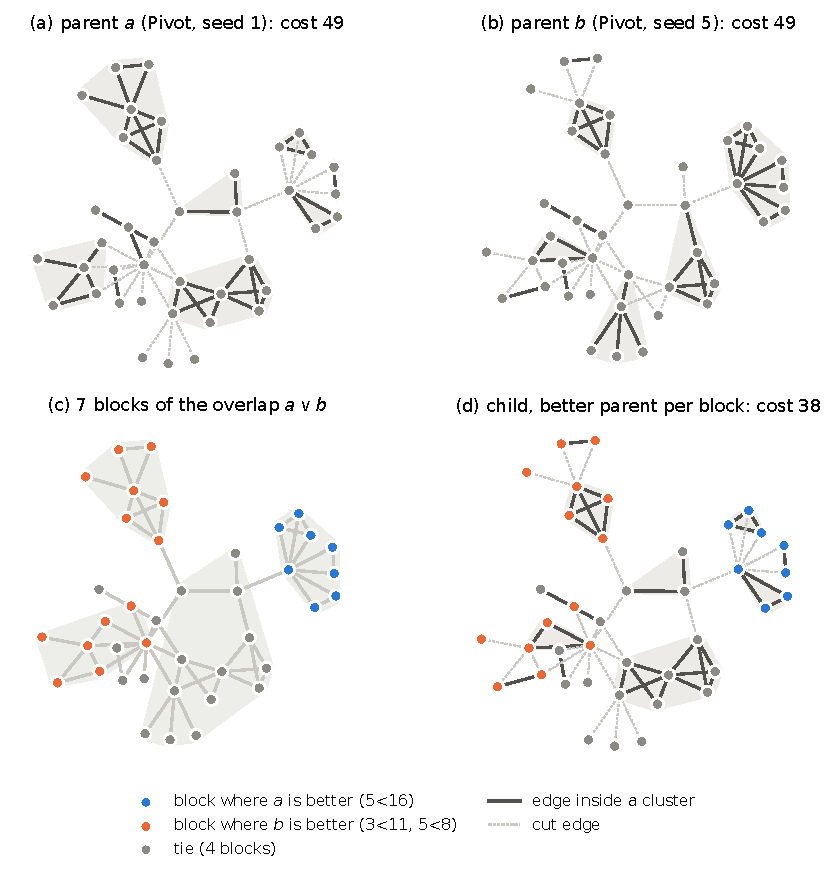
\includegraphics[width=0.88\textwidth]{figures/fig_crossover.pdf}
\caption{Partition crossover (Theorem~\ref{thm:px}) computed by the released
code.  (a), (b): two Pivot clusterings of the neighbourhood of
Figure~\ref{fig:support}, both of cost 49; shaded regions are clusters.
(c): the connected components of the overlap graph $H$ split the vertices into
seven blocks, and on each block the two parents can be compared on their own.
(d): taking the better parent on every block gives a clustering of cost 38,
better than both parents.}\label{fig:crossover}
\end{figure}

\begin{theorem}[partition crossover]\label{thm:px}
Let the cost of a clustering be any sum of pair terms that depend only on
whether the two vertices of the pair share a cluster (this covers $\cost$ and
the weighted cost~\eqref{eq:wcost}).  Let $a$ and $b$ be clusterings and let
$H$ be the bipartite graph whose nodes
are the clusters of $a$ and of $b$, with an edge between $A\in a$ and $B\in b$
whenever $A\cap B\ne\emptyset$.  Each connected component of $H$ covers a
vertex set $X$, the \emph{block}, which is a union of clusters of $a$ and also
a union of clusters of $b$.  For a clustering $c$ let $\cost_X(c)$ count the
mistakes on the pairs inside $X$.  Choose, independently in every block, the
clusters of $b$ if $\cost_X(b)<\cost_X(a)$ and those of $a$ otherwise.  The
resulting clustering $\chi$ satisfies
\[
\cost(\chi)=\cost(a)-\sum_X\max\bigl(0,\cost_X(a)-\cost_X(b)\bigr)
\le\min\bigl(\cost(a),\cost(b)\bigr).
\]
\end{theorem}
\begin{proof}
A pair $u,v$ in different blocks is separated by $a$, by $b$ and by $\chi$,
because each of their clusters lies inside one block.  It therefore
contributes the same amount to all three costs.  A pair inside a block $X$ is
treated by $\chi$ exactly as by the parent chosen for $X$.  Summing over the
pairs gives the equality.  Every term of the sum is non-negative, and
exchanging the roles of $a$ and $b$ gives the bound by $\cost(b)$.
\end{proof}

The blocks are the connected components of a bipartite graph with at most $n$
edges, and the block costs need one pass over $\Ep$.  Hence $\chi$ is computed in
$O(n+m)$ time.  The blocks form the join $a\vee b$ of the two partitions in the partition
lattice: the finest partition whose parts are unions of clusters of $a$ and
also of $b$.  It is the finest partition for which every block-wise choice
between the parents yields each parent as one of the choices and leaves the
pairs between blocks separated in both.  Decomposing two parents into independent components and taking the better
parent in each is the partition crossover of
\citet{WhitleyHH09gpx,WhitleyHH10hybrid,TinosWO20gpx2} for tours and of
\citet{TinosWC15px} for pseudo-Boolean functions; recombination through the
overlap of groups is common in grouping genetic
algorithms~\citep{Falkenauer98grouping,GalinierH99coloring}, memetic graph
partitioning and clustering~\citep{SandersS12kaffpae,BiedermannHSS18memetic}
and ensemble clustering~\citep{OvelgonneG13ensemble}, and fusion
moves~\citep{BeierHK15fusion} combine proposals optimally within a restricted
space.  Theorem~\ref{thm:px} combines \emph{any} two clusterings, including
clusterings produced by different solvers.  On our graphs, two independent runs typically differ in thousands of
blocks, most of them ties, and each run wins some of the others.

\subsection{Annealing moves}

The search moves nodes of the contracted instance.  Let $S_X=\sum_{K\in X}s_K$
be the size of a cluster $X$ and $w(K,X)=\sum_{L\in X\setminus\{K\}}w_{KL}$.
Moving a node $K$ of size $s$ from its cluster $A$ to a cluster $B$ changes
$\cost_w$ by
\begin{equation}\label{eq:move}
\delta=s\,(S_B-S_A+s)+2\,\bigl(w(K,A)-w(K,B)\bigr).
\end{equation}
Exchanging $K\in A$ with $L\in B$ changes it by the sum of two such terms,
where the second one uses $S_A-s_K$, $S_B+s_K$, $w(L,B)+w_{KL}$ and
$w(L,A)-w_{KL}$.  Both are evaluated in $O(\deg K+\deg L)$ time.  The
simulated annealing~\citep{KirkpatrickGV83} proposes the move to the cluster
of a random neighbour, the best move, or a move to a new cluster, and accepts
with the Metropolis rule under a geometric cooling schedule.  It records the
best state with an undo journal, so a new best state costs $O(1)$ instead of
a copy of the labelling.  This alone made the annealing $7.3$ times faster on
\texttt{com-Amazon}.

\paragraph{Region-wise acceptance.}  Theorem~\ref{thm:px} turns annealing into
an iterated local search with a decomposed acceptance test.  From the current
clustering $x$ we anneal a copy, starting at a raised temperature, down to its
final state $y$, and set $x\gets\chi(x,y)$.  Every block in which $y$ improved
on $x$ is kept, even if $y$ is worse overall, and the cost of $x$ never
increases.

\paragraph{Localized annealing with rollback.}  A step grows a region of at
most $30$ nodes by breadth-first search around a centre, anneals only the
nodes of the region from a high to a low temperature, finishes with greedy best
moves, and undoes all moves if their total change is positive.  The undo is
exact: moves are reversed in LIFO order together with the free list of
cluster labels.  Half of the centres are drawn with probability proportional to
the degree.  Comparing our solutions with those of KaPoCE block by block showed
why: the blocks in which KaPoCE was better all contained a vertex of high
degree.

\subsection{The memetic search}

\begin{algorithm}[t]
\caption{PXMem$(G^+,T)$}\label{alg:pxmem}
\begin{algorithmic}[1]
\State contract the critical cliques
\For{$i=1,\dots,4$}
  \State $p_i\gets\textsc{Pivot}(G^+)$; $f_i\gets$ one round of \textsc{IteratedFlip}$(p_i)$
  \State $x_i\gets$ the cheaper of $p_i$ and $f_i$ on the contracted nodes; anneal $x_i$
\EndFor
\While{time remains}
  \State choose an operator by an $\varepsilon$-greedy bandit on the recent gain per second
  \State \textbf{crossover:} parents $a,b$ by binary tournaments; $z\gets\chi(a,b)$;
  \Statex \hspace{\algorithmicindent} contract the blocks common to $a$ and $b$ and run a multilevel local search from $z$;
  \Statex \hspace{\algorithmicindent} anneal on the nodes where $a$ and $b$ disagree; accept region-wise; crowding replacement
  \State \textbf{PX-annealing step} on a member (temperature chosen by a second bandit)
  \State \textbf{localized annealing} with rollback on a member
\EndWhile
\State \Return the cheapest member, expanded to $V$
\end{algorithmic}
\end{algorithm}

Algorithm~\ref{alg:pxmem} keeps a population of four clusterings.  A crossover
child enters the population only by replacing a member that is not cheaper,
preferring the most similar members (crowding); the other two operators
replace a member only if they improve it.  Contracting the blocks common to
both parents and continuing with a multilevel search from the recombined
clustering follows the recombination of memetic graph partitioners and
clusterers~\citep{SandersS12kaffpae,BiedermannHSS18memetic,hausberger2025scc}.  The flipping round of line~3 costs a few
full local-search passes whatever its time limit; with budgets below
\SI{300}{s} the seeds are therefore Pivot clusterings only, and no further seed
is generated once half of the budget is used.

\begin{theorem}\label{thm:pxmem}
Let $\mathcal C$ be the output of Algorithm~\ref{alg:pxmem} and $p_1$ the first
Pivot clustering.  Then $\cost(\mathcal C)\le\cost(p_1)$ for every outcome of
the random choices, and hence $\mathbb E[\cost(\mathcal C)]\le3\,\OPT$.  Together
with a lower bound $\LB$ from Section~\ref{sec:dual},
$\cost(\mathcal C)/\lceil\LB\rceil$ bounds the ratio achieved on the instance.
\end{theorem}
The guarantee is inherited from the Pivot seed, as for any procedure that
starts from a Pivot clustering and never makes its best solution worse; we state
it because every operator of the search must respect it, and this is what the
formal development checks.

\begin{proof}
The seed $x_1$ costs at most $\cost(p_1)$: Pivot does not separate twins, so its
contraction preserves its cost, and $x_1$ is the cheaper of the two
candidates.  The annealing returns the cheapest state of a trajectory that
starts at its input; region-wise acceptance does not increase the cost by
Theorem~\ref{thm:px}; the localized annealing keeps a step only if its total
change is non-positive; and every replacement is by a clustering that is not
more expensive than the member it replaces.  By induction over the
replacements, some member always costs at most $\cost(x_1)$, so the cheapest
final member costs at most $\cost(p_1)$.  Taking expectations and applying the
Pivot guarantee~\citep{AilonCN08} gives the second claim.  The last claim is
Theorem~\ref{thm:anytime}(a).
\end{proof}


\subsection{Comparison with KaPoCE}\label{sec:exp-h2h}

\paragraph{Protocol.}  PXMem and KaPoCE are compared under a
protocol that was fixed before the runs
(\texttt{experiments/heldout.md}).  On one machine, the two solvers run one
after the other in an order drawn from a hash of (graph, seed), each on the
same logical core while the machine is otherwise idle.  Both read the same
PACE-format text file inside their measured time.  KaPoCE's only changes are
a seed and its two internal time limits, set to $\tfrac{590}{600}T$ and
$\tfrac{90}{600}T$ (the ratio of its PACE configuration); it is stopped with
SIGTERM at $T$ and its output is validated.  PXMem is scored at KaPoCE's
elapsed wall-clock time, read from its improvement history, so the
comparison is at equal elapsed time; its value at $T$ is also recorded.
Invalid KaPoCE output counts as a PXMem win, as in PACE, and is reported
separately.  Budgets are $T=\SI{600}{s}$ (primary), \SI{150}{s} and
\SI{60}{s}, with ten seeds on each held-out SNAP graph and one run on each
PACE heuristic instance at \SI{600}{s}.

\paragraph{Statistics.}  The unit of inference is the graph.  For each graph
we take the median over seeds of the relative difference
$(\cost_{\mathrm{PXMem}}-\cost_{\mathrm{KaPoCE}})/\cost_{\mathrm{KaPoCE}}$ and
apply the two-sided Wilcoxon signed-rank test~\cite{Wilcoxon45} and the sign
test to the twelve medians.  Per graph we report the exact sign test over
seeds with Holm's correction~\cite{Holm79} over graphs, noting that with ten
seeds only a 10:0 split can be significant, and the Hodges--Lehmann
estimate~\cite{HodgesL63} of the paired difference with its exact confidence
interval.  We do not claim equivalence from non-significance.  Performance
profiles~\cite{DolanM02profiles} summarise the PACE heuristic track.


\begin{table}[!tbp]
\centering
\caption{PXMem against KaPoCE on the twelve held-out SNAP graphs,
$T=\SI{600}{s}$ (primary budget), ten seeds per graph.  W/T/L: runs in
which PXMem is better, equal, worse.  median, HL: median and Hodges--Lehmann
estimate of $(\cost_{\mathrm{PXMem}}-\cost_{\mathrm{KaPoCE}})/
\cost_{\mathrm{KaPoCE}}$ in percent, negative when PXMem is better, with the
exact $95\%$ confidence interval; $p$: exact sign test over the seeds;
$p_{\mathrm{Holm}}$: Holm-adjusted over the twelve graphs.  Last row: the
pre-registered tests over the twelve graph medians.}
\label{tab:h2h-600}
\footnotesize
\setlength{\tabcolsep}{4pt}
\pending{}

\end{table}

\begin{table}[!tbp]
\centering
\caption{As Table~\ref{tab:h2h-600}, $T=\SI{150}{s}$.}
\label{tab:h2h-150}
\footnotesize
\setlength{\tabcolsep}{4pt}
\begin{tabular}{lrcrlrr}
\toprule
graph & runs & W/T/L & median (\%) & HL (\%) [95\% CI] & $p$ & $p_{\mathrm{Holm}}$ \\
\midrule
\texttt{email-Eu-core} & 6 & 0/5/1 & $+0.000$ & $+0.000$ [$+0.000$, $+0.008$] & 1.000 & 1.000 \\
\texttt{facebook} & 6 & 0/6/0 & $+0.000$ & $+0.000$ [$+0.000$, $+0.000$] & 1.000 & 1.000 \\
\texttt{wiki-Vote} & 6 & 5/0/1 & $-0.008$ & $-0.007$ [$-0.016$, $+0.026$] & 0.219 & 1.000 \\
\texttt{cit-HepTh} & 5 & 4/0/1 & $-0.009$ & -- & 0.375 & 1.000 \\
\texttt{cit-HepPh} & 6 & 3/0/3 & $-0.000$ & $-0.000$ [$-0.021$, $+0.039$] & 1.000 & 1.000 \\
\texttt{p2p-Gnutella31} & 6 & 0/4/2 & $+0.000$ & $+0.000$ [$+0.000$, $+0.001$] & 0.500 & 1.000 \\
\texttt{soc-Slashdot0902} & 6 & 0/0/6 & $+0.006$ & $+0.007$ [$+0.004$, $+0.010$] & 0.031 & 0.375 \\
\texttt{loc-Gowalla} & 5 & 0/0/5 & $+0.008$ & -- & 0.062 & 0.688 \\
\texttt{email-EuAll} & 5 & 5/0/0 & $-0.011$ & -- & 0.062 & 0.688 \\
\texttt{amazon0302} & 5 & 0/0/5 & $+0.008$ & -- & 0.062 & 0.688 \\
\texttt{web-NotreDame} & 5 & 0/0/5 & $+0.022$ & -- & 0.062 & 0.688 \\
\texttt{roadNet-PA} & 4 & 0/0/4 & $+0.507$ & -- & 0.125 & 0.875 \\
\midrule
\multicolumn{7}{l}{graph medians: 4 better, 3 equal, 5 worse; Wilcoxon $p=0.652$, sign test $p=1.000$} \\
\bottomrule
\end{tabular}

\end{table}

\begin{table}[!tbp]
\centering
\caption{As Table~\ref{tab:h2h-600}, $T=\SI{60}{s}$.}
\label{tab:h2h-60}
\footnotesize
\setlength{\tabcolsep}{4pt}
\pending{}

\end{table}

\paragraph{Primary budget.}  At \SI{600}{s} (Table~\ref{tab:h2h-600},
\numHHSixRuns{} paired runs) the graph medians favour PXMem on
\numHHSixBetter{} graphs and KaPoCE on \numHHSixWorse{}, with
\numHHSixEqual{} ties.  Neither pre-registered test rejects equality of the
two solvers (Wilcoxon $p=\numHHSixWilcoxon$, sign test
$p=\numHHSixSign$).  After Holm's correction PXMem is better on
\texttt{loc-Gowalla} and KaPoCE on \texttt{amazon0302} and
\texttt{roadNet-PA}; PXMem wins nine of ten seeds on \texttt{wiki-Vote},
\texttt{cit-HepTh} and \texttt{cit-HepPh}, which is not significant after the
correction.  All differences are small: the largest graph median is
\numHHSixMaxAbs{}, and on the held-out graphs with a certificate the
certified gap of the best solution is at least \numSnapGapMinHeld{}
(Table~\ref{tab:snap-bounds}).  The certificates therefore cannot separate
the two solvers, and neither solver is shown to be near-optimal on these
graphs beyond what Table~\ref{tab:snap-bounds} certifies.  KaPoCE returned a
valid solution in every run (\numHHSixForfeitK{} forfeits).  Scoring PXMem at
$T$ instead of at KaPoCE's elapsed time gives \numHHSixAtTBetter{} better and
\numHHSixAtTWorse{} worse graph medians (Wilcoxon $p=\numHHSixAtTWilcoxon$).
Many per-seed differences are zero or tied on some graphs
(\texttt{email-Eu-core}, \texttt{facebook}, \texttt{p2p-Gnutella31}); there
the Hodges--Lehmann interval degenerates and its coverage is not exact, and
zero graph medians are dropped from the Wilcoxon test, which the analysis
plan did not specify.  We do not claim that the two solvers are
equivalent: the study was not designed as an equivalence test.

\paragraph{Shorter budgets.}  KaPoCE did not stop by itself and was
terminated by SIGTERM in \numHHSixSigterm{}, \numHHOneFiftySigterm{} and
\numHHSixtySigterm{} of the 120 runs at \SI{600}{s}, \SI{150}{s} and
\SI{60}{s}; it then writes its best solution, which can take some seconds,
while PXMem is scored at KaPoCE's elapsed time.  This favours KaPoCE.  At
\SI{150}{s} (Table~\ref{tab:h2h-150}) the picture is similar (\numHHOneFiftyBetter{} better, \numHHOneFiftyEqual{}
equal, \numHHOneFiftyWorse{} worse; Wilcoxon $p=\numHHOneFiftyWilcoxon$),
with larger losses of PXMem on the largest graphs, up to
\numHHOneFiftyMaxAbs{} on \texttt{roadNet-PA}.  At \SI{60}{s}
(Table~\ref{tab:h2h-60}) KaPoCE is better on \numHHSixtyWorse{} of the
\numHHSixtyGraphs{} graph medians (Wilcoxon $p=\numHHSixtyWilcoxon$).  PXMem is
a population method, and a short budget leaves few recombinations on graphs
with $10^5$ vertices or more; we did not analyse this further.  PXMem is thus
not a replacement for KaPoCE at short budgets, and at the primary budget the
two are not distinguishable by our tests.

\paragraph{PACE heuristic track.}  On the 200 instances of the PACE~2021
heuristic track, one run per instance at \SI{600}{s} under the same protocol,
the instance is the unit.  The \numPDn{} instances that coincide with
development graphs are reported separately (Table~\ref{tab:pace-heur}).  On
the other \numPHn{} instances PXMem is better on \numPHBetter{}, equal on
\numPHEqual{} and worse on \numPHWorse{} (Wilcoxon $p=\numPHWilcoxon$, sign
test $p=\numPHSign$); KaPoCE returned no valid solution on
\numPHKapoceInvalid{} instances, which count as PXMem wins as in PACE.
The counts hide the sizes of the differences: summed over the \numPHn{}
instances the costs favour KaPoCE by 5185, and the eleven instances with
$10^5$ vertices or more contribute 5344 of this (PXMem better on six of
them, worse on five).
PXMem records its first solution only after its initialisation; on
\numPHNoSolution{} small instance KaPoCE stopped before that, and it
counts as a KaPoCE win under the protocol.
Figure~\ref{fig:profile} shows the performance profile.

\begin{table}[!tbp]
\centering
\caption{PACE~2021 heuristic track, $T=\SI{600}{s}$, one run per instance:
PXMem against KaPoCE by instance size.  W/T/L: instances on which PXMem is
better, equal, worse; $\sum$: total difference of the costs; median: of the
relative differences in percent.}
\label{tab:pace-heur}
\footnotesize
\begin{tabular}{l}
\pending{} (54 of 200 runs done)
\end{tabular}

\end{table}

\begin{figure}[!tbp]
\centering
\IfFileExists{figures/profile_pace_heur.pdf}{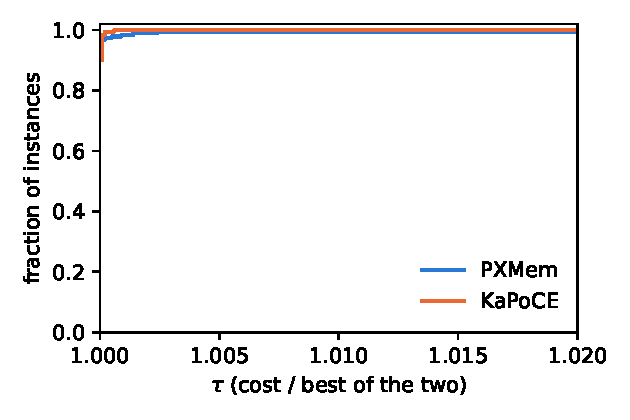
\includegraphics[width=0.6\textwidth]{figures/profile_pace_heur.pdf}}{\pending{}}
\caption{Performance profile~\cite{DolanM02profiles} on the PACE heuristic
track without the development twins: fraction of instances on which a
solver's cost is within a factor $\tau$ of the better of the two.}
\label{fig:profile}
\end{figure}
